\section{Webclient} \label{sec:Webclient}
In diesem Abschnitt wird zuerst auf den Unterschied zwischen Multi Page Applications und Single Page Applications eingegangen, um eine Architektur für die neue Weboberfläche zu wählen. Im Anschluss wird das Design unter Zuhilfenahme von Mockups erläutert.

\subsection{SPA vs MPA} \label{subsec:SPA_vs_MPA}

\paragraph{Multi Page Applications} \label{para:Multi_Page_Applications}
Multi Page Application, kurz MPA, ist die klassische Architektur für Webanwendungen. Bei dieser Architektur wird für jeden Request (Anfrage) an den Webserver eine neue Seite inklusive Ressourcen wie Cascading Style Sheets (CSS)\footnote{Beinhalten Regeln für die Darstellung von unter anderem HTML-Dokumenten}, JavaScript und Bildern geladen. Dieses kann an einem Beispiel verdeutlicht werden.

Auf einer Shop-Seite befinden sich 10 Produkte inkl. Bild und Kurzbeschreibung. Wird ein Produkt ausgewählt, sendet der Client eine Anfrage an den Webserver. Der Webserver antwortet mit allen Ressourcen (siehe oben), die für das Produkt benötigt werden. Der Client stellt dann aus den Ressourcen die Ansicht dar und das Produkt inklusive der Details ist für die Nutzenden zu sehen.

Der Vorteil von MPAs ist die einfachere Optimierbarkeit für Suchmaschinen, das sogenannte SEO (Search Engine Optimization). Ein gutes SEO-Rating sorgt dafür, dass die Webseite bei Suchmaschinen weit oben zu finden ist. Dies ist besonders für Webseiten wichtig, die um Kunden konkurrieren. Anzuführen sind hier diverse Online-Shops und Zeitungen.

\paragraph{Single Page Applications} \label{para:Single_Page_Applications}
Die Single Page Application, kurz SPA, stellt das genaue Gegenteil von MPAs dar. Bei SPAs besteht die Anwendung aus genau einem HTML-Dokument, dessen Inhalt bei Bedarf dynamisch nachgeladen wird. Dafür findet ein asynchroner Datenaustausch zwischen Client und Server statt, bei dem benötigte Ressourcen wie Bilder, JavaScript und CSS ausgetauscht werden. Durch dieses Verfahren wird sichergestellt, dass gleiche Elemente oder Ressourcen nicht erneut heruntergeladen werden müssen. Bei Änderungen werden nur Teile des DOMs\footnote{Das Document Object Model repräsentiert die Webseite als Baumstruktur} ersetzt und neu gerendert.

Die Interaktion mit dem DOM oder auch Virtual DOM kann selbst entwickelt werden. Jedoch ist hierbei zu raten, auf bereits bestehende Frameworks wie Angular (Entwickelt unter der Leitung vom Angular Team bei Google), React (Entwickelt unter der Leitung von Facebook) oder Vue (Evan You und Core Team) zurückzugreifen. 

Der große Vorteil von SPAs ist die Geschwindigkeit der Anwendung, da hier nur einzelne Teile ausgetauscht werden müssen. SPAs bieten außerdem den Vorteil, dass die Entwicklung von Front- und Backend entkoppelt wird. Das heißt, dass die Programmierenden des Front- und Backends weitestgehend unabhängig voneinander arbeiten können.

Die SEO-Optimierung gestaltet sich schwieriger, da es sich um eine dynamische Anwendung handelt. Zur Nutzung von SPAs muss im Browser JavaScript in der benötigten Version verfügbar und aktiviert sein.

\clearpage
\paragraph{Zusammenfassung Vor- und Nachteile} \label{para:Zusammenfassung_Vor-_und_Nachteile}
\mbox{} % Damit die Tablle in der neuen Zeile angezeigt wird
\begin{center}
	\begin{tabular}{rcc}
		& SPA & MPA \\
		Vorteile &
		\begin{minipage}[t]{0.4\textwidth}
			\begin{itemize}
				\item Sehr schnell, dank dynamischem Nachladen
				\item Entkoppelung zwischen Front- und Backend
				\item Effizientes cachen von Daten
			\end{itemize}
		\end{minipage} &
		\begin{minipage}[t]{0.4\textwidth}
			\begin{itemize}
				\item MPA Architektur ist ausgereift
				\item MPAs sind entwicklerfreundlich, da ein kleiner Technologiestack benötigt wird
				\item Ältere Browser werden in der Regel unterstützt
				\item SEO ist einfacher zu implementieren
			\end{itemize}
		\end{minipage}\\
		& & \\ % Space zwischen Vor- und Nachteilen
		Nachteile &
		\begin{minipage}[t]{0.4\textwidth}
			\begin{itemize}
				\item JavaScript muss in der benötigten Version im Browser verfügbar sein
				\item Alte Browser werden nur teilweise unterstützt
				\item Herausfordernde SEO Implementierung
			\end{itemize}
		\end{minipage} &
		\begin{minipage}[t]{0.4\textwidth}
			\begin{itemize}
				\item Anwendungen sind weniger performant als SPAs
				\item Front- und Backend haben eine starke Kopplung
			\end{itemize}
		\end{minipage}
	
	\end{tabular}
\label{tab:Vor-_und_Nachteile_SPA/MPA}
\end{center}

Bei der Entwicklung der Anwendung entscheide ich mich für die Verwendung einer SPA. Dies geschieht unter den Gesichtspunkten der Entkopplung zwischen Front- und Backend, der Performance der Anwendung und der Zukunftssicherheit, die meiner Meinung nach für SPAs besteht. Die Nachteile vom SPAs betreffen meine Anwendung nur wenig. So ist auf den Rechnern im Labor ein moderner Webbrowser installiert und in diesem JavaScript aktiviert. Auch handelt es sich um eine interne Anwendung, bei der die SEO Optimierung keine Rolle spielt. \cite{melnikSinglePageApplication2020}

\subsection{Mockups} \label{subsec:Mockup}

Für das Layout der Oberfläche wird die Designsprache Material Design von Google verwendet, da dieses konkrete Gestaltungsregeln vorgibt und einen Styleguide zur Verfügung stellt. Material Design wurde im Jahr 2014 vorgestellt und in Apps von Google verwendet. Besonders die Optimierung der Benutzerfreundlichkeit steht im Vordergrund. Eine Besonderheit des Material Designs ist, dass physikalische Gesetze beachtet werden und die Inhalte für eine Priorisierung auf einer virtuellen Z-Ebene verschoben werden. \cite{kulturbanause-teamMaterialDesignDesignsprache2017}

Den Prinzipien des Dark Theme von Material Design wird gefolgt, da die bestehende Anwendung bereits nur im Dark Mode vorhanden ist. Derzeit werden Anwendungen häufig mit Dark Mode als Default Theme veröffentlicht und bestehende Anwendungen ohne Dark Mode erhalten diesen als zusätzliches Farbschema. \cite{colbyWindows10Dark2020}

Das Dark Themes trägt zur Verbesserung der visuellen Ergonomie bei, was zu einer Reduktion der Belastung der Augen führt. Bei OLED-Bildschirmen wird die Batterieleistung geschont. Die im Light Theme verwendete Verschiebung auf der Z-Ebene wird durch Schatten erreicht und ist deshalb im Dark Theme nicht nutzbar. Anstatt eine Verschiebung vorzunehmen, werden die Elemente unterschiedlich beleuchtet.\cite{googleDarkTheme}

Damit die Icons zum Design der Seite passen und einheitlich sind, werden Material Design Icons\footnote{\url{https://materialdesignicons.com/}} verwendet. Hier sind die offiziellen Icons sowie Icons von der Community, die dem Material Design Ansatz folgen, vorhanden.

\begin{center}
	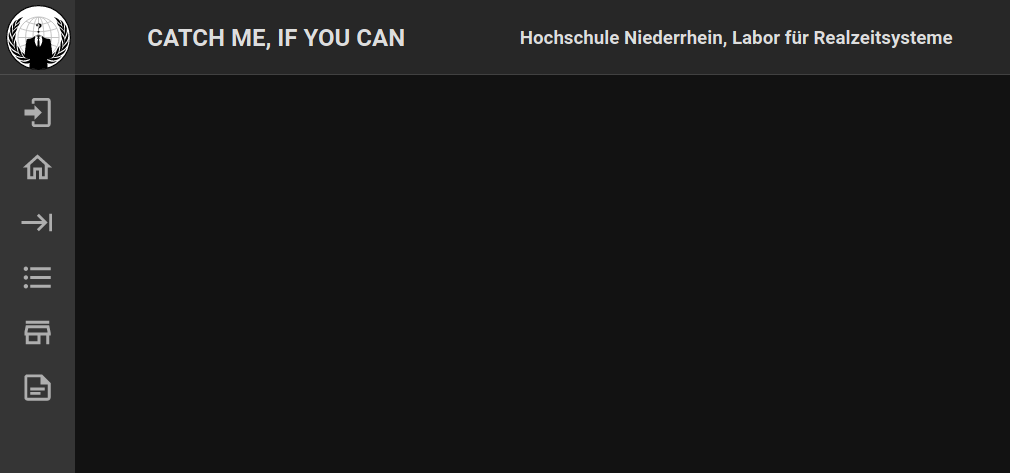
\includegraphics[width=\linewidth]{entwurf/webclient/base}
	\captionof{figure}{Grundlayout der Weboberfläche (Mockup)}
	\label{fig:mockup-base}
\end{center}

Das Grundlayout ist wie in \autoref{fig:mockup-base} dargestellt in drei Bereiche, Header (1), Navigation (2) und Content (3), eingeteilt. 

Der Bereich des Headers ist im oberen Teil erkennbar. Dort sind ein Logo, derzeitig noch das Logo aus der alten Anwendung, eine Überschrift sowie ein Untertitel platziert. Über die Überschrift und den Untertitel können die verschieden Seiten (Admin-, Spieler-, Flagshop- und Challengeseite) unterscheidbar gemacht werden.

Die Navigation ist auf der linken Seite erkennbar und als Sidebar mit Icons realisiert. Diese beinhaltet Verweise zu den Unterseiten. Sollte ein Eintrag der Navigation aktiv sein, wird dieser mithilfe der im Material Design vorgesehenen Farbe hervorgehoben.

Der Rest der Seite ist der Content Bereich. Dieser wird dynamisch mit dem anzuzeigenden Inhalt gefüllt.

\begin{center}
	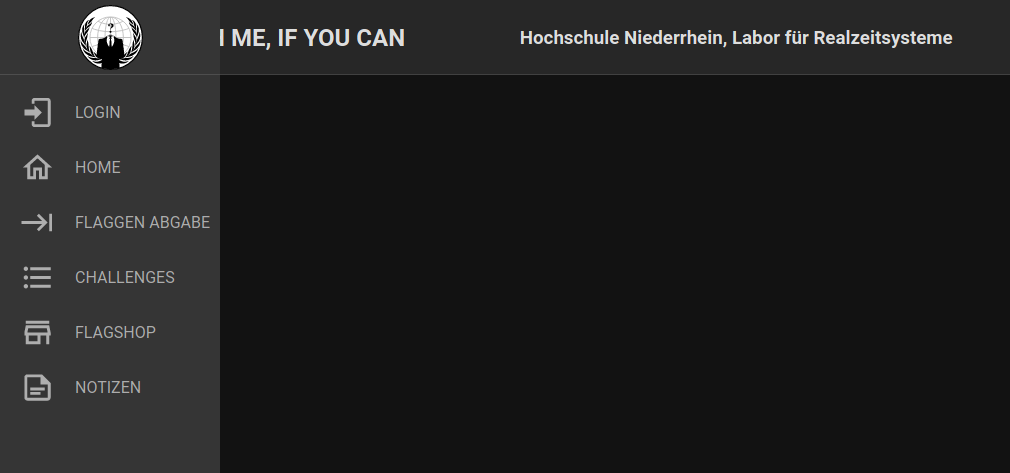
\includegraphics[width=\linewidth]{entwurf/webclient/base-extended}
	\captionof{figure}{Ausgeklapptes Menü beim drüberfahren (Mockup)}
	\label{fig:mockup-base-extended}
\end{center}

Damit die Navigation verständlich wird, gibt es wie in \autoref{fig:mockup-base-extended} zu erkennen neben den Icons auch beschreibenden Text. Dieser Text wird angezeigt, wenn der Nutzende mit der Maus über die Sidebar fährt. Die Sidebar wird über den Content ausgefahren und überdeckt diesen.

\begin{center}
	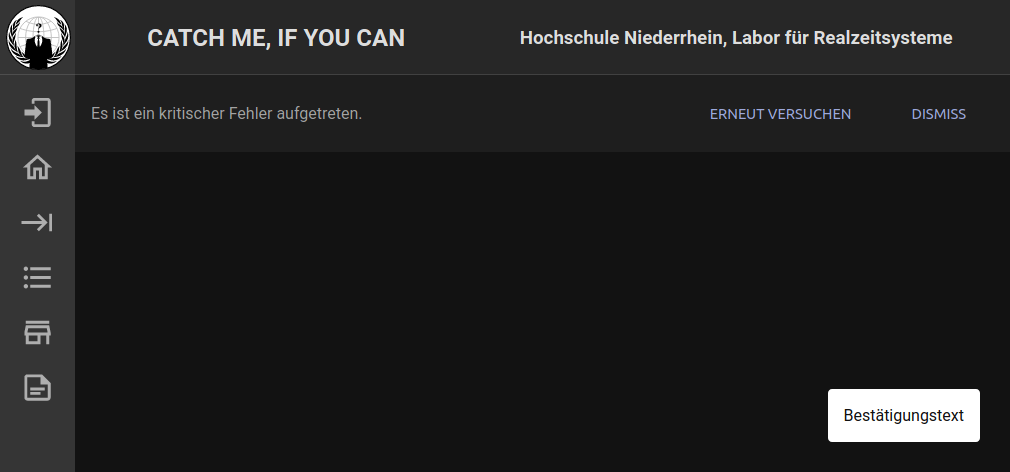
\includegraphics[width=\linewidth]{entwurf/webclient/base-with-error}
	\captionof{figure}{Fehlernachrichten (Mockup)}
	\label{fig:mockup-base-with-error}
\end{center}

Sollte der Nutzende über Ereignisse informiert werden, stehen zwei Möglichkeiten zur Verfügung.

Wenn das Ereignis wichtig ist, wird ein Banner verwendet. Dieser Banner besteht aus drei Elementen, einem Element für die Nachricht und zwei Buttons. Der linke der beiden ermöglicht es dem Nutzenden eine Aktion direkt auszuführen. Dies kann unter anderem eine Weiterleitung zu einer bestimmten Seite sein, über die der Nutzende weitere Informationen erhält. Über den anderen Button kann der Banner ausgeblendet werden. Es wird maximal ein Banner zeitgleich angezeigt.

Die andere Möglichkeit den Nutzenden zu informieren, ist die sogenannte Snackbar. Diese wird verwendet, wenn die Benutzererfahrung nicht unterbrochen werden soll und keine Benutzereingabe benötigt wird.
Die Snackbar wird am  unteren rechten Rand platziert und verschwindet im Gegensatz zum Banner nach einer definierten Zeit automatisch. Wenn möglich wird auch hier maximal eine Snackbar gleichzeitig verwendet.

\begin{minipage}{\textwidth}
	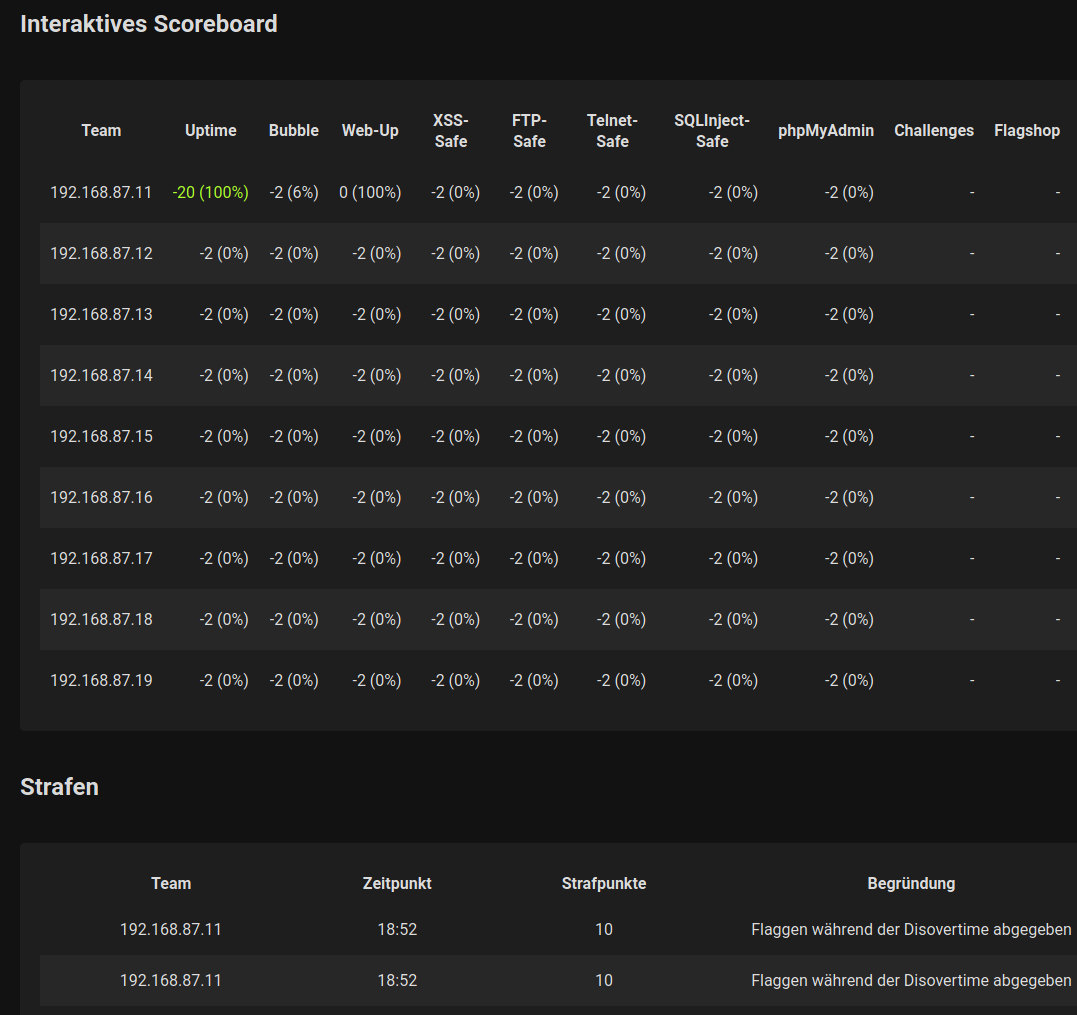
\includegraphics[width=\linewidth]{entwurf/webclient/table}
	\captionof{figure}{Ansicht des Spielstandes (Mockup)}
	\label{fig:mockup-table}
\end{minipage}

In \autoref{fig:mockup-table} ist ein Teil der Ansicht des Interaktiven Scoreboards inklusive der Strafen abgebildet. Die Ansicht ist in das Grundlayout der Anwendung (\autoref{fig:mockup-base}) eingebettet. Wie bereits oben erwähnt wird die Tabelle, um diese vom Hintergrund abzusetzen, unter Zuhilfenahme einer helleren Farbe dargestellt. Damit die Zeilen in der Tabelle besser erkennbar sind, ist jede zweite Zeile hervorgehoben. 

Dienste, die beim letzten Scan den gewünschten Zustand hatten, werden mit einem kontrastarmen grün dargestellt. Im Gegensatz zu der vorhanden Anwendung wird auf eine rote Darstellung der Dienste, bei unerwünschtem Zustand, verzichtet. Einzig die Gesamtpunkte werden im negativen Bereich rot dargestellt.
